\RequirePackage{currfile}
\documentclass[12pt]{beamer}
\usepackage[utf8]{inputenc}
\usepackage[spanish]{babel}
\usepackage{standalone}
\usepackage{color}
\usepackage{siunitx}
\usepackage{hyperref}
%\hypersetup{colorlinks,linkcolor=,urlcolor=blue}
%\hypersetup{colorlinks,urlcolor=blue}
\usepackage{xcolor,soul}
\usepackage{etoolbox}
\usepackage{amsmath}
\usepackage{amsthm}
\usepackage{physics}
\usepackage{multicol}
\usepackage{bookmark}
\usepackage{longtable}
\usepackage{listings}
\usepackage{graphicx}
\usepackage{tikz}
\usetikzlibrary{patterns, matrix, backgrounds, decorations,shapes, arrows.meta}
\usepackage[autostyle,spanish=mexican]{csquotes}
\usepackage[os=win]{menukeys}
\usepackage{pifont}
\usepackage{pbox}
\usepackage{caption}
\captionsetup{font=scriptsize,labelfont=scriptsize}
%\usepackage[sfdefault]{roboto}  %% Option 'sfdefault' only if the base font of the document is to be sans serif

%Sección de definición de colores
\definecolor{ao}{rgb}{0.0, 0.5, 0.0}
\definecolor{bisque}{rgb}{1.0, 0.89, 0.77}
\definecolor{amber}{rgb}{1.0, 0.75, 0.0}
\definecolor{armygreen}{rgb}{0.29, 0.33, 0.13}
\definecolor{alizarin}{rgb}{0.82, 0.1, 0.26}
\definecolor{cadetblue}{rgb}{0.37, 0.62, 0.63}
\definecolor{deepblue}{rgb}{0,0,0.5}
\definecolor{brown}{rgb}{0.59, 0.29, 0.0}
\definecolor{OliveGreen}{rgb}{0,0.25,0}


\usefonttheme[onlymath]{serif}
%Sección de definición de nuevos comandos

\newcommand*{\TitleParbox}[1]{\parbox[c]{1.75cm}{\raggedright #1}}%
\newcommand{\python}{\texttt{python}}
\newcommand{\textoazul}[1]{\textcolor{blue}{#1}}
\newcommand{\azulfuerte}[1]{\textcolor{blue}{\textbf{#1}}}
\newcommand{\funcionazul}[1]{\textcolor{blue}{\textbf{\texttt{#1}}}}
\newcommand{\ptilde}[1]{\ensuremath{{#1}^{\prime}}}
\newcommand{\stilde}[1]{\ensuremath{{#1}^{\prime \prime}}}
\newcommand{\ttilde}[1]{\ensuremath{{#1}^{\prime \prime \prime}}}
\newcommand{\ntilde}[2]{\ensuremath{{#1}^{(#2)}}}
\renewcommand{\arraystretch}{1.5}

\newcounter{saveenumi}
\newcommand{\seti}{\setcounter{saveenumi}{\value{enumi}}}
\newcommand{\conti}{\setcounter{enumi}{\value{saveenumi}}}
\renewcommand{\rmdefault}{cmr}% cmr = Computer Modern Roman

\linespread{1.5}

\usefonttheme{professionalfonts}
%\usefonttheme{serif}
\DeclareGraphicsExtensions{.pdf,.png,.jpg}


%Sección para el tema de beamer, con el theme, usercolortheme y sección de footers
\mode<presentation>
{
  \usetheme{Warsaw}
  
  %\useoutertheme{infolines}
  \useoutertheme{default}
  \usecolortheme{spruce}
  \setbeamercovered{invisible}
  % or whatever (possibly just delete it)
  \setbeamertemplate{section in toc}[sections numbered]
  \setbeamertemplate{subsection in toc}[subsections numbered]
  \setbeamertemplate{subsection in toc}{\leavevmode\leftskip=3.2em\rlap{\hskip-2em\inserttocsectionnumber.\inserttocsubsectionnumber}\inserttocsubsection\par}
  \setbeamercolor{section in toc}{fg=blue}
  \setbeamercolor{subsection in toc}{fg=blue}
  \setbeamercolor{frametitle}{fg=blue}
  \setbeamertemplate{caption}[numbered]

  \setbeamertemplate{footline}
  \beamertemplatenavigationsymbolsempty
  \setbeamertemplate{headline}{}
}

\makeatletter
\setbeamercolor{section in foot}{bg=gray!30, fg=black!90!orange}
\setbeamercolor{subsection in foot}{bg=blue!30!yellow, fg=red}
\setbeamertemplate{footline}
{
  \leavevmode%
  \hbox{%
  \begin{beamercolorbox}[wd=.333333\paperwidth,ht=2.25ex,dp=1ex,center]{section in foot}%
    \usebeamerfont{section in foot} \insertsection
  \end{beamercolorbox}}%
  \begin{beamercolorbox}[wd=.333333\paperwidth,ht=2.25ex,dp=1ex,center]{subsection in foot}%
    \usebeamerfont{subsection in foot}  \insertsubsection
  \end{beamercolorbox}%
  \begin{beamercolorbox}[wd=.333333\paperwidth,ht=2.25ex,dp=1ex,right]{date in head/foot}%
    \usebeamerfont{date in head/foot} \insertshortdate{} \hspace*{2em}
    \insertframenumber{} / \inserttotalframenumber \hspace*{2ex} 
  \end{beamercolorbox}}%
  \vskip0pt%
\makeatother  

\makeatletter
\patchcmd{\beamer@sectionintoc}
  {\vfill}
  {\vskip\itemsep}
  {}
  {}
\makeatother


\title{\large{Diferenciales y operadores diferenciales}}
\subtitle{Tema 1 - La física y la geometría}
\author{M. en C. Gustavo Contreras Mayén}
\date{\today}
\institute{Facultad de Ciencias - UNAM}
\titlegraphic{
\includegraphics[width=1.75cm]{../Imagenes/escudo-facultad-ciencias}\hspace*{4.75cm}~%
   
\includegraphics[width=1.75cm]{../Imagenes/escudo-unam}
}
\setbeamertemplate{navigation symbols}{}
\begin{document}
\maketitle
\fontsize{14}{14}\selectfont
\spanishdecimal{.}
\section*{Contenido}
\frame{\tableofcontents[currentsection, hideallsubsections]}
\section{Diferencial de línea}
\frame{\tableofcontents[currentsection, hideothersubsections]}
\subsection{Construcción}
\begin{frame}
\frametitle{Construcción}
Utilizando el resultado
\begin{align*}
\vu{e}_{i} = \dfrac{1}{h_{i}} \, \pdv{\vb{r}}{u_{i}}
\end{align*}
en la ecuación inicial
\begin{align*}
\dd{\vb{r}} = \sum_{i=1}^{3} \pdv{\vb{r}}{u_{i}} \dd{u_{i}}
\end{align*}
\end{frame}
\begin{frame}
\frametitle{Diferencial de línea}
Es posible escribir:
\begin{align}
\dd{\vb{r}} = \sum_{i=1}^{3} h_{i} \, \vu{e}_{i} \dd{u_{i}} = \sum_{i=1}^{3} \dd{\vb{l}_{i}}
\label{eq:ecuacion_01_21}
\end{align}
\pause
donde
\begin{align}
\dd{\vb{l}_{i}} = h_{i} \, \vu{e}_{i} \dd{u_{i}}
\label{eq:ecuacion_01_22}
\end{align}
que representa el \emph{elemento diferencial de línea} a lo largo del eje $u_{i}$.
\end{frame}
\begin{frame}
\frametitle{Diferencia de línea}
La ec. (\ref{eq:ecuacion_01_22}) asegura que cualquier elemento de línea con orientación arbitraria, puede descomponerse en una suma vectorial.
\end{frame}
\subsection*{Coordenadas esféricas}
\begin{frame}
\frametitle{Coordenadas esféricas}
En coordenadas esféricas tenemos que:
\begin{table}
\begin{tabular}{r  c  l}
$\dd{\vb{l}_{r}} = \vu{e}_{r} \dd{r}$ & $\longrightarrow$ & $\dd{l_{r}} = \dd{r}$ \\
$\dd{\vb{l}_{\theta}} = \vu{e}_{\theta} \, r \dd{\theta}$ & $\longrightarrow$ & $\dd{l_{\theta}} = r \, \dd{\theta}$ \\
$\dd{\vb{l}_{\varphi}} = \vu{e}_{\varphi} \, r \, \sin \theta \dd{\varphi}$ & $\longrightarrow$ & $\dd{l_{\varphi}} = r \, \sin \theta \dd{\varphi}$ \\
\end{tabular}
\end{table}
\end{frame}
\section{Diferencial de superficie}
\frame{\tableofcontents[currentsection, hideothersubsections]}
\subsection{Construcción}
\begin{frame}
\frametitle{Construción}
Las superficies diferenciales se describen como vectores perpendicular al área diferencial, como se ve en la siguiente figura (\ref{fig:figura_diferenciales_superficie}):
\end{frame}
\begin{frame}
\frametitle{Diferenciales de superficie}
\begin{figure}[h!]
    \centering
    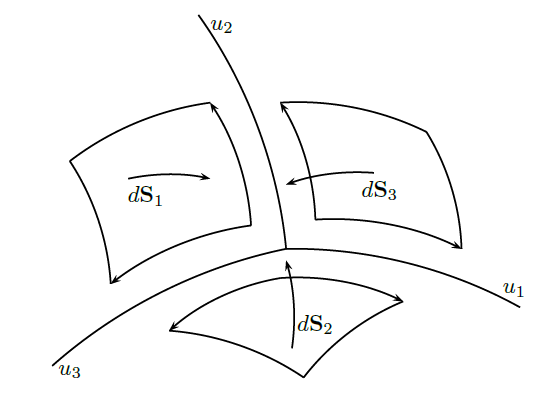
\includegraphics[scale=0.5]{Imagenes/Diferenciales_Superficie_01.png}
    \caption{Elementos diferenciales de área en coordenadas curvilíneas.}
    \label{fig:figura_diferenciales_superficie}
\end{figure}
\end{frame}
\begin{frame}
\frametitle{Diferenciales de superficie}
Las superficies están orientadas según la regla de la mano derecha, por lo que:
\begin{align*}
\dd{\vb{S}_{1}} &= \dd{\vb{l}_{2}} \cp \dd{\vb{l}_{3}} \\[0.5em] 
\dd{\vb{S}_{2}} &= \dd{\vb{l}_{3}} \cp \dd{\vb{l}_{1}} \\[0.5em]
\dd{\vb{S}_{3}} &= \dd{\vb{l}_{1}} \cp \dd{\vb{l}_{2}}
\end{align*}
\end{frame}
\begin{frame}
\frametitle{Usando un resultado previo}
Usando las relaciones:
\begin{align*}
\vu{e}_{1} \cp \vu{e}_{2} = \vu{e}_{3} \\
\vu{e}_{2} \cp \vu{e}_{3} = \vu{e}_{1} \\
\vu{e}_{3} \cp \vu{e}_{1} = \vu{e}_{2}
\end{align*}
que son válidas para sistemas coordenados curvilíneos ortonormales, en espacios 3D euclidianos.
\end{frame}
\begin{frame}
\frametitle{Usando un resultado previo}
Que en forma sintética queda expresado por:
\begin{align}
\vu{e}_{i} \cp \vu{e}_{j} = \sum_{i=1}^{3} \epsilon_{ijk} \, \vu{e}_{k}
\end{align}
donde $\epsilon_{ijk}$ es el símbo de \emph{Levi-Civita} que definimos en la presentación anterior.
\end{frame}
\begin{frame}
\frametitle{Diferenciales de superficie}
Así encontramos que
\begin{align*}
\dd{\vb{S}_{1}} &= h_{2} \, h_{3} \, \vu{e}_{2} \cp \vu{e}_{3} \dd{u_{2}} \dd{u_{3}} = \\[0.5em]
&= h_{2} \, h_{3} \, \vu{e}_{1} \dd{u_{2}} \dd{u_{3}} = \\[0.5em]
&= \vu{e}_{1} \dd{S_{1}}
\end{align*}
\end{frame}
\begin{frame}
\frametitle{Superficies diferenciales}
Para los otros dos diferenciales de superficie:
\fontsize{12}{12}\selectfont
\begin{eqnarray*}
\dd{\vb{S}_{2}} &=& h_{3} \, h_{1} \, \vu{e}_{3} \cp \vu{e}_{1} \dd{u_{3}} \dd{u_{1}} = \\[0.5em]
&=& h_{3} \, h_{1} \, \vu{e}_{2} \dd{u_{3}} \dd{u_{1}} = \\[0.5em]
&=& \vu{e}_{2} \dd{S_{2}} \\[1em]
\pause
\dd{\vb{S}_{3}} &=& h_{1} \, h_{2} \, \vu{e}_{1} \cp \vu{e}_{2} \dd{u_{1}} \dd{u_{2}} = \\[0.5em]
&=& h_{1} \, h_{2} \, \vu{e}_{3} \dd{u_{1}} \dd{u_{2}} = \\[0.5em]
&=& \vu{e}_{3} \dd{S_{3}}
\end{eqnarray*}
\end{frame}
\section{Diferencial de volumen}
\frame{\tableofcontents[currentsection, hideothersubsections]}
\subsection{Construcción}
\begin{frame}
\frametitle{Construcción}
El elemento diferencial de volumen se define como
\begin{align*}
\dd{V} &= \dd{\vb{l}_{1}} \cdot \dd{\vb{l}_{2}} \cp \dd{\vb{l}_{3}} = \\
&= h_{1} \, h_{2} \, h_{3} \, \vu{e}_{1} \cdot \vu{e}_{2} \cp \vu{e}_{3} \dd{u_{1}} \dd{u_{2}} \dd{u_{3}} = \\
&= h_{1} \, h_{2} \, h_{3} \dd{u_{1}} \dd{u_{2}} \dd{u_{3}}
\end{align*}
\end{frame}
\subsection*{Coordenadas esféricas}
\begin{frame}
\frametitle{Coordenadas esféricas}
En coordenadas esféricas tenemos:
\begin{align*}
\dd{S_{1}} &= \dd{S_{r}} = h_{\theta} \, h_{\varphi} \dd{\theta} \dd{\varphi} = r^{2} \sin \theta \dd{\theta} \dd{\varphi} \\[0.5em]
\dd{S_{2}} &= \dd{S_{\theta}} = h_{\varphi} \, h_{r} \dd{\varphi} \dd{r} = r \sin \theta \dd{\theta} \dd{\varphi} \\[0.5em]
\dd{S_{3}} &= \dd{S_{\varphi}} = h_{r} \, h_{\theta} \dd{r} \dd{\theta} = r \dd{r} \dd{\theta}
\end{align*}
\end{frame}
\begin{frame}
\frametitle{Construcción}
Entonces el diferencial de volumen es:
\begin{align*}
\dd{V} &= h_{r} \, h_{\theta} \, h_{\varphi} \dd{r} \dd{\theta} \dd{\varphi} = \\[0.5em]
&= r^{2} \, \sin \theta \dd{r} \dd{\theta} \dd{\varphi}
\end{align*}
\end{frame}
\begin{frame}
\frametitle{Ejercicio a cuenta}
La velocidad y la aceleración se definen en la forma vectorial como:
\begin{align*}
\vb{v} = \dv{\vb{r}}{t} = \dot{\vb{r}} \hspace{1cm} \vb{a} = \dot{\vb{v}} = \ddot{\vb{r}}
\end{align*}
Calcula:
\setbeamercolor{item projected}{bg=blue!70!black,fg=yellow}
\setbeamertemplate{enumerate items}[circle]
\begin{enumerate}
\item $\dot{\vu{e}}_{r}$, $\dot{\vu{e}}_{\theta}$, $\dot{\vu{e}}_{\varphi}$ 
\item La velocidad $\vb{v}$
\item La aceleración $\vb{a}$
\end{enumerate}
\end{frame}
\begin{frame}
\frametitle{Ejercicio a cuenta}
Demuestra que para dos vectores $\vb{A}$ y $\vb{B}$:
\setbeamercolor{item projected}{bg=blue!70!black,fg=yellow}
\setbeamertemplate{enumerate items}[circle]
\begin{enumerate}
\item $\vb{A} \cp \vb{B} = \displaystyle \sum_{ijk} \, \vu{e}_{i} \, \epsilon_{ijk} \, A_{j} \, B_{k}$ \\[1em]
\item $\vb{A} \cdot \vb{B} \cp \vb{C} = \displaystyle \sum_{ijk} \, \epsilon_{ijk} \, A_{i} \, B_{j} \, C_{k}$
\end{enumerate}
\end{frame}
\section{Operadores diferenciales}
\frame{\tableofcontents[currentsection, hideothersubsections]}
\begin{frame}
\frametitle{Sobre los campos escalares y vectoriales}
En la presentación anterior mencionamos la naturaleza de los campos escalares y vectoriales.
\\
\bigskip
\pause
Asumiremos que los campos son funciones regulares, continuas y derivables, excepto posiblemente en algunos puntos aislados.
\end{frame}
\begin{frame}
\frametitle{Sobre los campos escalares y vectoriales}
En general los campos serán descritos por ecuaciones diferenciales parciales cuyas variables independientes serán la posición y el tiempo
\end{frame}
\subsection{Gradiente}
\begin{frame}
\frametitle{El gradiente}
Al pasar de un punto 
\begin{align*}
P(u_{1}, u_{2}, u_{3})
\end{align*}
a otro infinitesimalmente cercano 
\begin{align*}
P(u_{1} + \dd{u}_{1}, u_{2} + \dd{u_{2}} + u_{3} + \dd{u_{3}})
\end{align*}
\end{frame}
\begin{frame}
\frametitle{El gradiente}
El cambio diferencial de una función (o campo) escalar $\phi(u_{1}, u_{2}, u_{3})$ está dado por:
\begin{align}
\begin{aligned}
\dd{\phi} &= \pdv{\phi}{u_{1}} \dd{u_{1}} + \pdv{\phi}{u_{2}} \dd{u_{2}} + \pdv{\phi}{u_{3}} \dd{u_{3}} \\[0.5em]
&= \sum_{i=1}^{3} \pdv{\phi}{u_{i}} \dd{u_{i}}
\end{aligned}
\label{eq:ecuacion_01_26}
\end{align}
\end{frame}
\begin{frame}
\frametitle{El gradiente}
Teniendo en cuenta la ec. (\ref{eq:ecuacion_01_21}) se sigue que:
\begin{align}
\dd{\vb{r}} = \sum_{j=1}^{3} h_{j} \, \vu{e}_{j} \dd{u_{j}}
\label{eq:ecuacion_01_27}
\end{align}
\pause
Multiplicando escalarmente por $\vu{e}_{i}$ tenemos que:
\end{frame}
\begin{frame}
\frametitle{El gradiente}
\begin{align*}
\dd{\vb{r}} \cdot \vu{e}_{i} &= \sum_{j=1}^{3} h_{j} \, \vu{e}_{j} \cdot \vu{e}_{j} \dd{u_{j}} = \sum_{j=1}^{3} h_{j} \, \delta_{ij} \dd{u_{j}} \\[0.5em]
&= h_{i} \dd{u_{i}} \\[1em]
&\Longrightarrow \dd{u_{i}} = \dfrac{1}{h_{i}} \dd{\vb{r}} \cdot \vu{e}_{i}
\end{align*}
\end{frame}
\begin{frame}
\frametitle{El gradiente}
Al sustituir en la ec. (\ref{eq:ecuacion_01_26}), llegamos a:
\begin{align*}
\dd{\phi} &= \sum_{i=1}^{3} \pdv{\phi}{u_{i}} \, \dfrac{1}{h_{i}} \, \vu{e}_{i} \cdot \dd{\vb{r}} = \\[0.5em]
&= \dd{\vb{r}} \cdot \left( \sum_{i=1}^{3} \dfrac{\vu{e_{i}}}{h_{i}} \, \pdv{\phi}{u_{i}} \right)
\end{align*}
\pause
Al término entre paréntesis lo denotamos $\nabla{\phi}$.
\end{frame}
\begin{frame}
\frametitle{Definición del gradiente}
El operador \emph{nabla} es:
\begin{align}
\nabla{\phi} = \sum_{i=1}^{3} \dfrac{\vu{e_{i}}}{h_{i}} \, \pdv{\phi}{u_{i}} = \sum_{i=1}^{3} \vu{e}_{i} \left( \nabla{\phi} \right)_{i}
\label{eq:ecuacion_01_28}
\end{align}
\pause
Se le llamará \emph{gradiente de la función escalar} $\phi(u_{i})$, por tanto
\begin{align}
\dd{\phi} = \dd{\vb{r}} \cdot \nabla{\phi}
\label{eq:ecuacion_01_29}
\end{align}
\end{frame}
\begin{frame}
\frametitle{Derivada direccional}
Como tenemos que
\begin{align*}
\dd{\vb{r}} = \vu{n} \dd{l}
\end{align*}
\pause
Se sigue que:
\begin{align*}
\dv{\phi}{l} = \vu{n} \cdot \nabla{\phi}
\end{align*}
que corresponde a la definición de \emph{derivada direccional} de la función $\phi$ en la dirección de $\vu{n}$.
\end{frame}
\subsection{Propiedades del gradiente}
\begin{frame}
\frametitle{Superficies cercanas}
Para estudiar las propiedades del gradiente tomemos un par de superficies infinitesimalmente cercanas, sobre cada una de las cuales la función $\phi$ toma valores constantes e infinitesimalmente distintos: $\phi$ y $\phi + \dd{\phi}$.
\\
\bigskip
\pause
En la teoría de campos se les llama \emph{superficies equipotenciales}.
\end{frame}
\begin{frame}
\frametitle{Superficies equipotenciales}
\begin{figure}[h!]
    \centering
    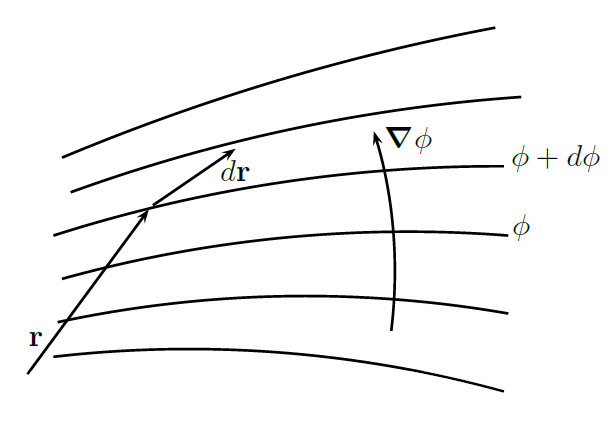
\includegraphics[scale=0.5]{Imagenes/Superficies_Equipotenciales.png}
    \caption{Superficies equipotenciales.}
    \label{fig:Superficies_Equipotenciales}
\end{figure}
\end{frame}
\begin{frame}
\frametitle{Propiedades del gradiente}
De la ec. (\ref{eq:ecuacion_01_29}) se tiene que:
\begin{align*}
\dd{\phi} = \dd{\vb{u}} \cdot \nabla{\phi} = \abs{\dd{\vb{r}}} \, \abs{\nabla{\phi}} \, \cos \theta
\end{align*}
donde $\theta$ es el ángulo entre $\dd{\vb{r}}$ y $\nabla{\phi}$.
\end{frame}
\begin{frame}
\frametitle{Propiedades del gradiene}
Si el vector $\dd{vb{r}}$ se sitúa en el plano $\phi = \mbox{ constante}$, entonces: $\dd{\phi} = =$, por lo que
\begin{align*}
0 = \abs{\dd{\vb{r}}} \, \abs{\nabla{\phi}} \, \cos \theta
\end{align*}
\pause
Como $\nabla{\phi}$ es en general diferente de cero, ya que $\phi(u_{i})$ es una función arbitraria, y como $\abs{\dd{\vb{r}}} \neq 0$, se sigue que $\cos \theta = 0$, entonces $\theta = \ang{90}$
\end{frame}
\begin{frame}
\frametitle{Propiedades del gradiente}
En consecuencia: $\nabla{\phi}$ es \emph{perpendicular} a la superficie $\phi = \mbox{ constante}$.
\\
\bigskip
\pause
El valor máximo de $\dd{\phi}$ se presenta cuando $\theta = 0$, es decir:
\begin{align*}
\dd{\theta}_{\max} &= \abs{\nabla{\phi}} \, \abs{\dd{\vb{r}}} \dd{l} \\[1em]
\mbox{o cuando } \hspace{0.5cm} \left( \dv{\phi}{l} \right)_{\max} &= \abs{\nabla{\phi}}
\end{align*}
\end{frame}
\begin{frame}
\frametitle{Módulo del gradiente}
Entonces el módulo del gradiente corresponde al valor máximo de la derivada direccional y el gradiente apunta en la dirección en que tal derivada es máxima.
\end{frame}
\begin{frame}
\frametitle{Construcción de sistema curvilíneos}
Dado que para cada punto de una línea o superficie equipotencial es posible trazar el vector $\nabla{\phi}$, entonces es posible construir una red coordenada ortogonal a las equipotenciales.
\end{frame}
\begin{frame}
\frametitle{Construcción de sistema curvilíneos}
Por lo que, dada una familia de curvas en el plano (o de superficies curvas en el espacio), es posible obtener otras que le sean ortogonales.
\end{frame}
\begin{frame}
\frametitle{Construcción de sistema curvilíneos}
Por lo que tenemos un método eficaz de construcción de sistemas de coordenadas curvilíneas ortogonales.
\end{frame}
\begin{frame}
\frametitle{Consideración importante}
Hay que tomar en cuenta que $\nabla$ \emph{no} es un vector, sino un \emph{operador vectorial}: $\nabla$ no tiene dirección, a menos que opere sobre una función.
\end{frame}
\begin{frame}
\frametitle{Ejercicios a cuenta}
Para ejercitar el avance que llevamos, resuelve:
\setbeamercolor{item projected}{bg=blue!70!black,fg=yellow}
\setbeamertemplate{enumerate items}[circle]
\begin{enumerate}
\item Demuestra que $\nabla{\phi \psi} = \phi \, \nabla{\psi} + \psi \, \nabla{\phi}$
\item Si $f = f(r)$ con $r = \sqrt{x^{2} + y^{2}+ z^{2}}$, demuestra que
\begin{align*}
\nabla{f(r)} = \vu{r} \, \dv{f(r)}{r}
\end{align*}
\end{enumerate}
\end{frame}
\section{Divergencia}
\frame{\tableofcontents[currentsection, hideothersubsections]}
\subsection{Flujo de campo vectorial}
\end{document}